\documentclass{article}

\usepackage{fancyhdr}
\usepackage{extramarks}
\usepackage{amsmath}
\usepackage{amsthm}
\usepackage{amsfonts}
\usepackage{tikz}
\usepackage[plain]{algorithm}
\usepackage{algpseudocode}
\usepackage[shortlabels]{enumitem}
\usepackage{listings}
\usepackage{color}




\definecolor{dkgreen}{rgb}{0,0.6,0}
\definecolor{gray}{rgb}{0.5,0.5,0.5}
\definecolor{mauve}{rgb}{0.58,0,0.82}

\lstset{ %
  language=R,                     % the language of the code
  basicstyle=\footnotesize,       % the size of the fonts that are used for the code
  numbers=left,                   % where to put the line-numbers
  numberstyle=\tiny\color{gray},  % the style that is used for the line-numbers
  stepnumber=1,                   % the step between two line-numbers. If it's 1, each line
                                  % will be numbered
  numbersep=5pt,                  % how far the line-numbers are from the code
  backgroundcolor=\color{white},  % choose the background color. You must add \usepackage{color}
  showspaces=false,               % show spaces adding particular underscores
  showstringspaces=false,         % underline spaces within strings
  showtabs=false,                 % show tabs within strings adding particular underscores
  frame=single,                   % adds a frame around the code
  rulecolor=\color{black},        % if not set, the frame-color may be changed on line-breaks within not-black text (e.g. commens (green here))
  tabsize=2,                      % sets default tabsize to 2 spaces
  captionpos=b,                   % sets the caption-position to bottom
  breaklines=true,                % sets automatic line breaking
  breakatwhitespace=false,        % sets if automatic breaks should only happen at whitespace
  title=\lstname,                 % show the filename of files included with \lstinputlisting;
                                  % also try caption instead of title
  keywordstyle=\color{blue},      % keyword style
  commentstyle=\color{dkgreen},   % comment style
  stringstyle=\color{mauve},      % string literal style
  escapeinside={\%*}{*)},         % if you want to add a comment within your code
  morekeywords={*,...}            % if you want to add more keywords to the set
}


\usetikzlibrary{automata,positioning}

%
% Basic Document Settings
%

\topmargin=-0.45in
\evensidemargin=0in
\oddsidemargin=0in
\textwidth=6.5in
\textheight=9.0in
\headsep=0.25in

\linespread{1.5}

\pagestyle{fancy}
\lhead{\hmwkAuthorName}
\chead{\hmwkClass\ (\hmwkClassInstructor): \hmwkTitle}
\rhead{\firstxmark}
\lfoot{\lastxmark}
\cfoot{\thepage}

\renewcommand\headrulewidth{0.4pt}
\renewcommand\footrulewidth{0.4pt}

\setlength\parindent{-5pt}

%
% Create Problem Sections
%

\newcommand{\enterProblemHeader}[1]{
    \nobreak\extramarks{}{Problem \arabic{#1} continued on next page\ldots}\nobreak{}
    \nobreak\extramarks{Problem \arabic{#1} (continued)}{Problem \arabic{#1} continued on next page\ldots}\nobreak{}
}

\newcommand{\exitProblemHeader}[1]{
    \nobreak\extramarks{Problem \arabic{#1} (continued)}{Problem \arabic{#1} continued on next page\ldots}\nobreak{}
    \stepcounter{#1}
    \nobreak\extramarks{Problem \arabic{#1}}{}\nobreak{}
}

\setcounter{secnumdepth}{0}
\newcounter{partCounter}
\newcounter{homeworkProblemCounter}
\setcounter{homeworkProblemCounter}{1}
\nobreak\extramarks{Problem \arabic{homeworkProblemCounter}}{}\nobreak{}

%
% Homework Problem Environment
%
% This environment takes an optional argument. When given, it will adjust the
% problem counter. This is useful for when the problems given for your
% assignment aren't sequential. See the last 3 problems of this template for an
% example.
%
\newenvironment{homeworkProblem}[1][-1]{
    \ifnum#1>0
        \setcounter{homeworkProblemCounter}{#1}
    \fi
    \section{Problem \arabic{homeworkProblemCounter}}
    \setcounter{partCounter}{1}\textbf{}
    \enterProblemHeader{homeworkProblemCounter}
}{
    \exitProblemHeader{homeworkProblemCounter}
}

%
% Homework Details
%   - Title
%   - Due date
%   - Class
%   - Section/Time
%   - Instructor
%   - Author
%

\newcommand{\hmwkTitle}{Problem Set 4}
\newcommand{\hmwkDueDate}{03/09}
\newcommand{\hmwkClass}{AMS 380.01}
\newcommand{\hmwkClassTime}{}
\newcommand{\hmwkClassInstructor}{Wei Zhu}
\newcommand{\hmwkAuthorName}{\textbf{Harris Temuri}}

%
% Title Page
%

\title{
    \vspace{2in}
    \textmd{\textbf{\hmwkClass:\ \hmwkTitle}}\\
    \normalsize\vspace{0.1in}\medium{Due\ on\ \hmwkDueDate}\\
    \vspace{0.1in}\large{\textit{\hmwkClassInstructor\ \hmwkClassTime}}
    \vspace{3in}
}

\author{\hmwkAuthorName}
\date{}

\renewcommand{\part}[1]{\textbf{\large Part \Alph{partCounter}}\stepcounter{partCounter}\\}

%
% Various Helper Commands
%

% Useful for algorithms
\newcommand{\alg}[1]{\textsc{\bfseries \footnotesize #1}}

% For derivatives
\newcommand{\deriv}[1]{\frac{\mathrm{d}}{\mathrm{d}x} (#1)}

% For partial derivatives
\newcommand{\pderiv}[2]{\frac{\partial}{\partial #1} (#2)}

% Integral dx
\newcommand{\dx}{\mathrm{d}x}

% Alias for the Solution section header
\newcommand{\solution}{\textbf{\large Solution}}

% Probability commands: Expectation, Variance, Covariance, Bias
\newcommand{\E}{\mathrm{E}}
\newcommand{\Var}{\mathrm{Var}}
\newcommand{\Cov}{\mathrm{Cov}}
\newcommand{\Bias}{\mathrm{Bias}}

\setlength{\jot}{1.5em}


\begin{document}

\maketitle

\pagebreak
    
\begin{homeworkProblem}
    You are a public health researcher interested in social factors that influence heart disease. You
    survey 498 towns and gather data on the percentage of people in each town who smoke, the
    percentage of people in each town who bike to work, and the percentage of people in each
    town who have heart disease. The dataset ‘heart.data.csv’ tabulates these variables.
    Is there a simple linear relationship between the percentage of people in each town who bike to
    work and the percentage of people in each town who have heart disease?

\textbf{\large{Solution}}
\begin{enumerate}[(a)]
    \item Find the least squares regression line.
    
    \begin{lstlisting}[belowskip=-1.5 \baselineskip]
    # 1.1 Finding Least squares regression line
    lin_fit <- lm(heart.disease ~ biking, data=heart_data)
    summary(lin_fit)
    \end{lstlisting}
 
    \[
        \textit{Heart Disease} = (-0.200297)*\textit{Biking} + 17.777880
    \]
 
    \item Plot the points and the regression line in the same figure.

    \begin{lstlisting}[belowskip=-1.5 \baselineskip]
    # 1.2 Plotting Linear Fit
    ggplot(data = heart_data, aes(x=biking, y=heart.disease)) + geom_point() + stat_smooth(method = lm)
    \end{lstlisting}
    
    \begin{figure}[h]
        \centering
        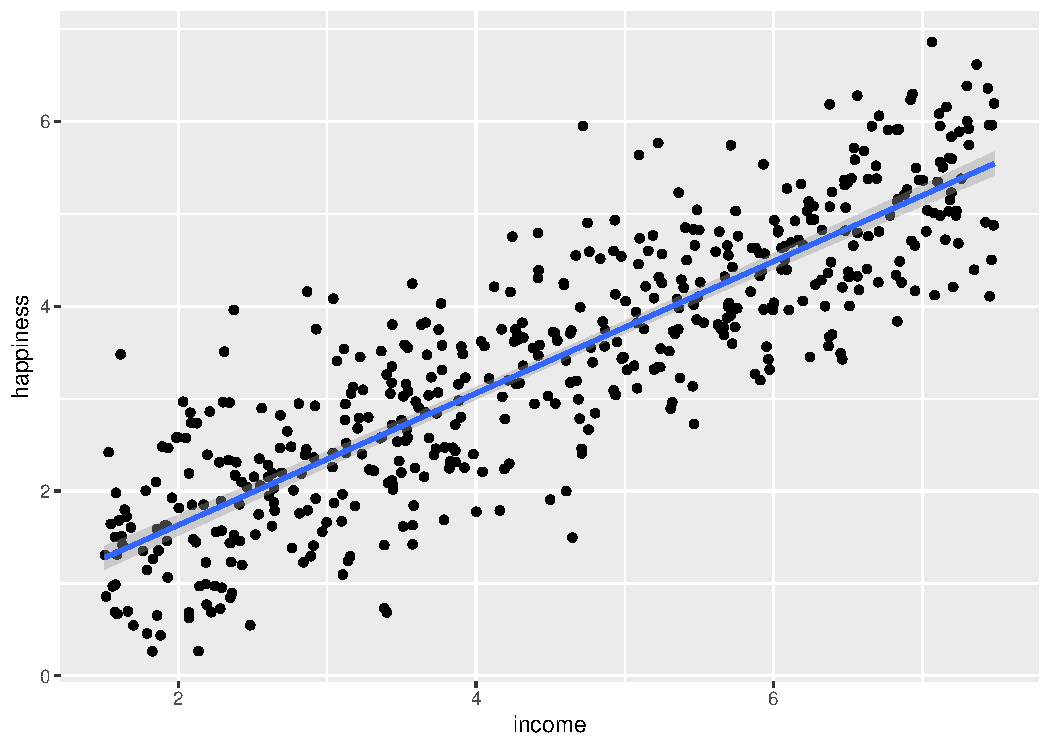
\includegraphics[scale = 0.7]{linReg_plot.pdf}
        \caption{Linear fit Biking vs Heart Disease}
        \label{fig:my_label}
    \end{figure}
    \newpage
    \item Test at $\alpha = 0.05$ whether there is a significant linear relationship between these two variables. 
    What assumptions are necessary? Please test these assumptions.
    \\

    \begin{lstlisting}[belowskip=-1.5 \baselineskip]
    # 1.3 Testing linear relationship along with assumptions
    # Normality Test of residuals
    shapiro.test(lin_fit$residuals)
    # Significance test (look at p-value of variable)
    summary(lin_fit)
    \end{lstlisting}
    
    The p-value of the normality test of the residuals is 0.4237 which is above 0.05 so do not reject the null hypothesis. 
    \\The p-value of the coefficient of biking in the linear regression is $<<$0.05 so the variable is significant.
    \\
    
    
    \item Compute the sample correlation coefficient between the two variables and test whether the
    corresponding population correlation is zero or not at $\alpha = 0.05$.
    
    \begin{lstlisting}[belowskip=-1.5 \baselineskip]
    # 1.4 Correlation coefficient test
    cor.test(heart_data$heart.disease, heart_data$biking)
    # Normality Test of variables
    shapiro.test(heart_data$heart.disease)
    shapiro.test(heart_data$biking)
    # Kendall Correlation Test
    cor.test(heart_data$heart.disease, heart_data$biking, method = "kendall")
    \end{lstlisting}
    
    The p-value of the Pearson test is $<<$0.05 so reject null hypothesis. There is significance between the variables happiness and income. 
    The sample correlation coefficient between the two variables is $-0.9753352$. The variables are not normal so its better to use Kendall 
    correlation test: p-value $<<$ 0.05, so reject null hypothesis, there is significant correlation between biking and heart disease.
    \\
    
    \item Report the coefficient of determination – does this statistic indicate a good linear model fit?
    (Note: Recall that for simple linear regression, the coefficient of determination is simply the 
    squared sample Pearson correlation coefficient.)
    
    \begin{lstlisting}[belowskip=-1.5 \baselineskip]
    # 1.5 Coefficient of determination
    cor(heart_data$heart.disease, heart_data$biking)^2
    \end{lstlisting}
    
    The value of the coefficient of determination is $0.9512788$.
\end{enumerate}
\end{homeworkProblem}
\newpage
%
%
%
% Problem 2
%
%
%

\begin{homeworkProblem}
    The data set ‘Diet.csv’ contains information on 76 people who undertook one of three diets in
    the hope of losing weight. There is also background information such as age, gender, and
    height. The aim of the study was to see which diet was best for losing weight. (*Note: please
    pay attention to the response variable we wish to analyze, which is weight loss – so you may
    need to generate this variable first from before you perform the analysis.)
\\

\textbf{\large{Solution}}
\begin{enumerate}[(a)]
    \item Please draw side-by-side box	plots to visually compare the yields from the three fertilizers.
    
    \begin{lstlisting}[belowskip=-1.5 \baselineskip]
    # 1.1 Box Plots of Diet effectiveness
    ggplot(data = Diet, aes(x = Diet, y = weight6weeks)) + geom_boxplot()
    \end{lstlisting}
    
    \begin{figure}[h]
        \centering
        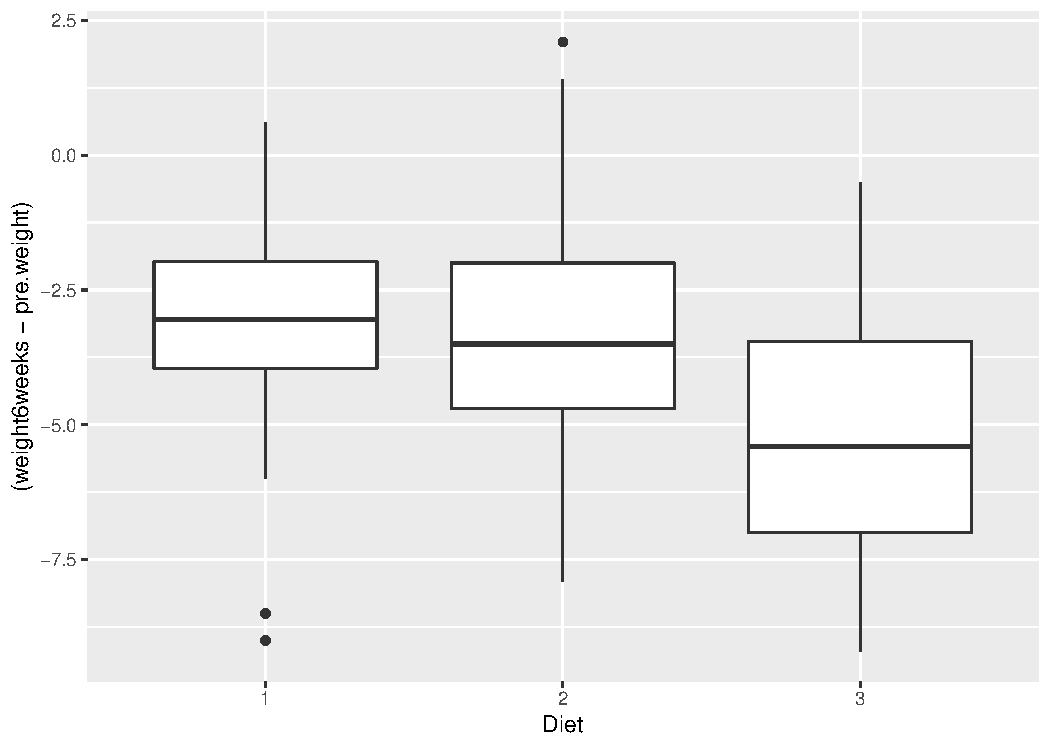
\includegraphics[scale = 0.8]{boxPlot1.pdf}
        \caption{Box Plot of Three Diets}
        \label{fig:my_label}
    \end{figure}
\newpage
    \item Test at $\alpha = 0.05$ whether the three diets are equally effective. What assumptions are necessary? Please test these assumptions. 
    
    \begin{lstlisting}
    # 1.2 Test for diets being equally effective
    res_aov <- aov(weight6weeks ~ Diet, data = Diet)
    summary(res_aov)
    # Testing Assumptions
    # Normality Test of residuals
    shapiro.test(res_aov$residuals)
    # Homogeneity of Variance test
    bartlett.test((weight6weeks-pre.weight) ~ factor(Diet), data = Diet)
    \end{lstlisting}
    
    Test for effectiveness: p-value $<<$ 0.05, so reject null hypothesis. They are not equally effective. Variance test: p-value less $>$ 0.05 so do not reject null hypothesis. 
    Variances are equal. Normality test: p-value $>$ 0.05 dont reject null hypothesis. The residuals are normal.

    \item At the familywise error rate of $\alpha = 0.05$, please perform pairwise comparison of the three 
    fertilizers using the Tukey HSD test.
    
    \begin{lstlisting}[belowskip=-1.5 \baselineskip]
    # 1.4 Tukey Test
    TukeyHSD(res_aov)
    \end{lstlisting}
    
    Group 2 and 1 is not significantly different; p-value $>$ 0.05
    \\Group 3 and 1 is significantly different; p-value $<$ 0.05
    \\Group 3 and 2 is significantly different; p-value $<$ 0.05
    
    \item Please compare diets 2 and 3 using the usual pooled-variance t-test at the significance 
    level  $\alpha = 0.05$. What assumptions are necessary? Please test these assumptions.
    
    \begin{lstlisting}[belowskip=-1.5 \baselineskip]
    # 1.5 Comparing Diets 2 and 3
    t.test((Diet$weight6weeks-Diet$pre.weight)[Diet$Diet == 2], (Diet$weight6weeks-Diet$pre.weight)[Diet$Diet == 3], var.equal = T)
    # Testing Assumptions
    # Normality of Groups
    shapiro.test((Diet$weight6weeks-Diet$pre.weight)[Diet$Diet == 2])
    shapiro.test((Diet$weight6weeks-Diet$pre.weight)[Diet$Diet == 3])
    # Var test
    var.test((Diet$weight6weeks-Diet$pre.weight)[Diet$Diet == 2], (Diet$weight6weeks-Diet$pre.weight)[Diet$Diet == 3])
    \end{lstlisting}
    
    Group 2 and 3 are significantly different because p $<$ 0.05 and we reject the null hypothesis. Both Diets are normal (p-value shapiro test $>$ 0.05). 
    Equal variances (var test p-value $>$ 0.05).

\end{enumerate}
\end{homeworkProblem}
\end{document}
